\begin{evenBlock}{Figure 8 Passing (10 min)}

\begin{minipage}[t]{\linewidth}
    \centering
    
    \begin{minipage}{.3\linewidth} % Left column and width
        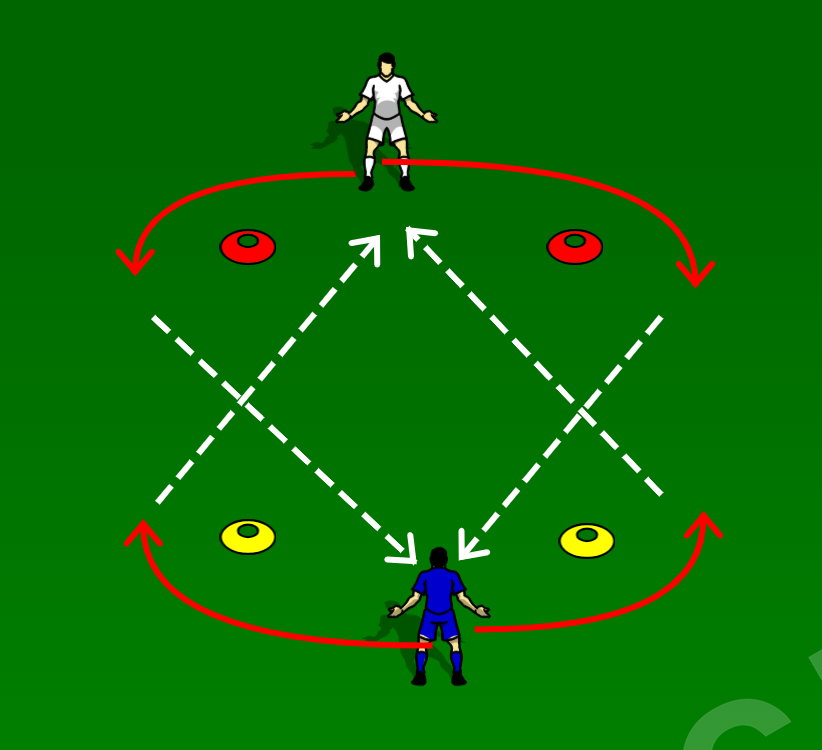
\includegraphics[width=\textwidth]{../img/Trimmed/Figure-8}
    \end{minipage}
    \hspace{0.05\linewidth}
    \begin{minipage}{.6\linewidth} % Left column and width
        \textbf{Drill Description:}
        This drill incorporates a lot of movement and passing.  Its designed to make the player trap and touch a ball around a defender for a clear pass.
        \begin{enumerate}
            \setlength{\itemsep}{0pt}
            \setlength{\parskip}{0pt}
            \setlength{\parsep}{0pt}
            \item Player 1 starts with the ball between two cones.  P2 starts between two cones the same width apart as P1 and 5 yards away.
            \item P1 dribbles around the cone on the right and passes to P2.
            \item P2 should trap the ball with the right foot and dribble around the right cone and pass to P1, who needs to race back between the two cones.
            \item This time P1 traps with the left foot and dribbles around the left cone and passes to P2.  P2 needs to race back between the two cones.
            \item P2 traps with the left and dribbles around the left cone to pass back to P1.
            \item At this point the drill repeats to the right side.
            \item After 10 passes stop and the P2 becomes the starting player.
        \end{enumerate}
    \end{minipage}
\end{minipage}

\textbf{Coaching Points:}
\begin{itemize}
    \setlength{\itemsep}{0pt}
    \setlength{\parskip}{0pt}
    \setlength{\parsep}{0pt}
    \item The cones are the defender, the goal is practice making that first touch and follow on touches into the open space then pass.
    \item Explain the first touch with the correct foot is important in guiding the ball into the open space.
    \item The goal would be able to use only 2 touches before making that third touch (the pass). 
    \item However I would rather see 3, 4 or 5 tight controlled touches than only 2 sloppy touches.

\end{itemize}


\end{evenBlock}